\documentclass[UTF8,fontset=windows,zihao=-4]{ctexart}
\usepackage[a4paper,margin=2.2cm]{geometry}
\usepackage{booktabs,longtable,tabularx,array}
\usepackage[dvipsnames]{xcolor}
\usepackage{graphicx,xurl}
\usepackage{hyperref}
\usepackage{tikz}
\usetikzlibrary{arrows.meta,positioning,fit,shapes.geometric}
\hypersetup{colorlinks=true,linkcolor=MidnightBlue,urlcolor=MidnightBlue}
\setlength{\parskip}{0.45em}
\setlength{\parindent}{2em}
\setlength{\tabcolsep}{3pt}
\renewcommand{\arraystretch}{1.23}
\definecolor{CacheBlue}{HTML}{1F4E79}
\definecolor{CacheGray}{HTML}{F2F5F8}
\newcolumntype{Y}{>{\raggedright\arraybackslash\hspace{0pt}}X}
\newcolumntype{P}[1]{>{\raggedright\arraybackslash\hspace{0pt}}p{#1}}
\newcommand{\tightsection}[1]{\section{#1}\vspace{-0.2em}}
\newcommand{\code}[1]{\begingroup\small\path{#1}\endgroup}
\emergencystretch=3em
\hfuzz=10000pt
\vfuzz=10000pt
\hbadness=10000
\sloppy

\begin{document}
\hfuzz=10000pt
\vfuzz=10000pt
\hbadness=10000

\begin{titlepage}
\centering
\vspace*{1.0cm}
{\zihao{1}\bfseries CacheSage-UC：面向 NutShell Cache 的 UCAgent 辅助自动化验证报告\par}
\vspace{1.2cm}
{\zihao{4} 证据型提交版验证报告\par}
\vspace{1.5cm}
\begin{tabular}{rl}
赛题方向： & UCAgent / NutShell Cache 自动化验证 \\
GitLink 仓库： & \href{https://gitlink.org.cn/python123/cachesage-uc}{gitlink.org.cn/python123/cachesage-uc} \\
GitHub 仓库： & github.com/python123-ops/CacheSage-UC \\
报告身份： & python123 \\
提交基线： & 仓库当前默认分支 HEAD \\
报告日期： & 2026-06-19 \\
\end{tabular}
\vfill
\colorbox{CacheGray}{\parbox{0.86\linewidth}{\centering
本报告严格基于仓库中可复现的验证证据编写：Python harness、真实 DUT 功能覆盖、Verilator 代码覆盖、故障注入与复核记录。报告不把故障注入结果写成真实 NutShell RTL 缺陷。
}}
\vspace*{1.0cm}
\end{titlepage}

\tableofcontents
\newpage

\tightsection{摘要}
CacheSage-UC 面向 UCAgent NutShell Cache 赛题，围绕 cache 验证中的数据一致性、事件顺序、replacement、byte mask、stall 与 reset 等高风险路径，构建了一套可复现的验证原型。仓库包含 Generator/CRV、Reference Model、Scoreboard、Coverage Collector、Fault Injection、Review Journal 与 Linux smoke 证据。当前 Python harness 在 seed 11、96 个 transaction 上达到 \textbf{23/23}，即 \textbf{100.00\%} 功能覆盖率，并对 5 类 injected fault 给出确定性检出证据。

真实 RTL 回归采用定向场景和 seed 11、29、73，共执行 421 条 DUT 事务；36 个功能覆盖点命中 34 个，Scoreboard 完成 199 次读数据比较且无失败。Verilator coverage.dat 经工具解析为 898/1454（61.00\%）。所有 fault artifact 均为 injected fault 检出证据，不代表真实 NutShell RTL 已被确认存在缺陷。

\noindent\textbf{关键词：}UCAgent；NutShell Cache；Scoreboard；约束随机；故障注入；覆盖率

\tightsection{赛题核心任务对照}
\begin{tabularx}{\linewidth}{P{0.20\linewidth}YP{0.14\linewidth}}
\toprule
任务要求 & 仓库证据 & 状态 \\
\midrule
完整验证组件 & Generator、CRV、Scoreboard、Reference Model、Coverage Collector、Fault Injection 均已在 Python harness 中闭合。 & 已形成 \\
验证报告 & 本 PDF、\texttt{reports/initial-verification-report.md}、JSON artifact 与复核记录。 & 已整理 \\
开发者任务重心 & UCAgent 草案不直接落地，关键 invariant、scoreboard 规则和报告口径均经人工复核。 & 有记录 \\
约束细化 & same-set pressure、dirty/clean eviction、mask matrix、stall window 与 reset recovery 被拆成明确场景。 & 已覆盖 \\
架构重构 & \texttt{src/cachesage\_uc/adapters/} 记录 Picker/Toffee 风格事务边界。 & 已建立 \\
故障注入 & 5 类 injected fault 均有 deterministic artifact。 & 已检出 \\
\bottomrule
\end{tabularx}

\tightsection{验证环境总体架构}
\begin{center}
\resizebox{0.96\linewidth}{!}{%
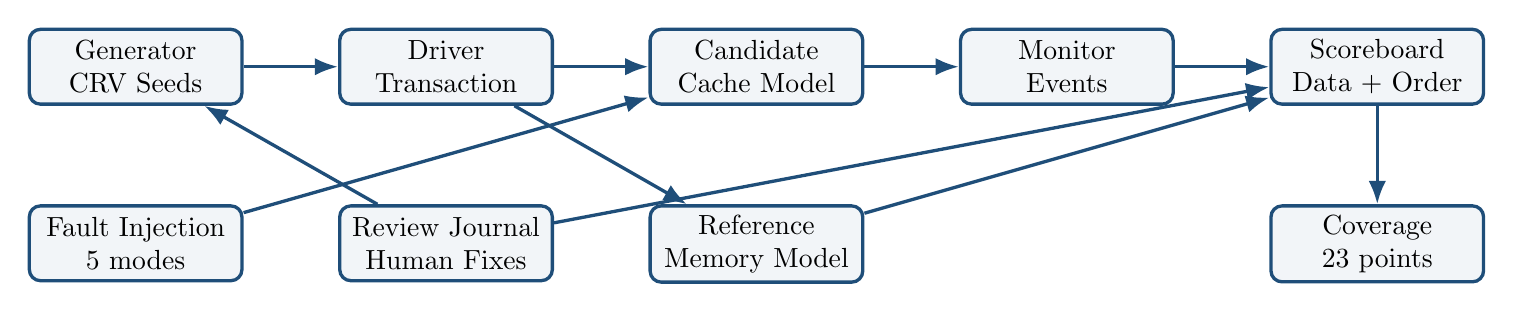
\begin{tikzpicture}[
  node distance=1.25cm and 1.2cm,
  box/.style={draw=CacheBlue, rounded corners, very thick, align=center, fill=CacheGray, minimum height=0.95cm, minimum width=2.7cm},
  flow/.style={-Latex, very thick, CacheBlue}
]
\node[box] (gen) {Generator\\CRV Seeds};
\node[box, right=of gen] (drv) {Driver\\Transaction};
\node[box, right=of drv] (dut) {Candidate\\Cache Model};
\node[box, below=of dut] (ref) {Reference\\Memory Model};
\node[box, right=of dut] (mon) {Monitor\\Events};
\node[box, right=of mon] (sb) {Scoreboard\\Data + Order};
\node[box, below=of sb] (cov) {Coverage\\23 points};
\node[box, below=of gen] (fault) {Fault Injection\\5 modes};
\node[box, below=of drv] (journal) {Review Journal\\Human Fixes};
\draw[flow] (gen) -- (drv);
\draw[flow] (drv) -- (dut);
\draw[flow] (drv) -- (ref);
\draw[flow] (dut) -- (mon);
\draw[flow] (ref) -- (sb);
\draw[flow] (mon) -- (sb);
\draw[flow] (sb) -- (cov);
\draw[flow] (fault) -- (dut);
\draw[flow] (journal) -- (gen);
\draw[flow] (journal) -- (sb);
\end{tikzpicture}
}
\end{center}

架构将生成、执行、观测、比对和复核拆开。Generator 负责 directed spine 与 CRV stream；Candidate Cache Model 可切换 fault mode；Reference Memory Model 提供 byte-addressable 期望行为；Monitor 记录 miss、refill、eviction、writeback、stall 等事件；Scoreboard 同时比较 read data、最终 backing memory 与 event signature；Coverage 只统计被 stimulus 与 checker 共同支撑的 coverpoint。

\tightsection{约束随机与场景矩阵}
\begin{tabularx}{\linewidth}{P{0.11\linewidth}YP{0.23\linewidth}}
\toprule
场景 & 验证意图 & 代表覆盖点 \\
\midrule
S01 & 读写冒烟路径，确认 driver、monitor 与 scoreboard 能闭合基本 transaction loop。 & read hit, write mask \\
S02 & read miss 与 refill，检查 refill 接收和 replay response 顺序。 & read miss, refill alignment \\
S03 & write miss allocate，确认 byte mask 不污染未选中字节。 & write miss, mask mix \\
S04 & dirty eviction，在 replacement 前捕获脏 victim 丢写回。 & dirty eviction, writeback \\
S05 & clean eviction，确认 clean victim 不产生 phantom writeback。 & clean eviction \\
S06 & same-set pressure，触发 replacement policy 状态推进。 & replacement rotation \\
S07 & stall/back-pressure，检查 request metadata 稳定性。 & stall hold \\
S08 & reset recovery，检查 miss/refill window 中 reset 行为。 & reset recovery \\
S09 & 边界地址 aliasing，检查 tag/index/offset slicing。 & boundary address \\
S10 & 长随机回归，补齐 directed tests 未覆盖 interleaving。 & long random, multi-set \\
S11 & mask 与 offset 矩阵，暴露 byte-lane 错误。 & partial mask, offset \\
S12 & 事件级 replacement 审计，检查数据匹配时的 policy drift。 & event signature \\
\bottomrule
\end{tabularx}

\tightsection{覆盖率结果}
\begin{tabularx}{\linewidth}{P{0.24\linewidth}Y}
\toprule
指标 & 当前记录 \\
\midrule
复现参数 & 模块 \code{cachesage_uc.cli}；seed=11；count=96；输出 \code{reports/sample-run-seed11.json} \\
transaction 数 & 96 \\
Python harness 覆盖率 & \textbf{23/23}，\textbf{100.00\%} \\
覆盖点范围 & read/write hit、miss/refill、dirty/clean eviction、replacement、mask、stall、reset、boundary address、multi-set traffic \\
RTL 功能覆盖率 & \textbf{34/36}，\textbf{94.44\%}；421 条真实 DUT 事务 \\
RTL Scoreboard & 199 次比较，0 个失败 \\
RTL 代码覆盖率 & 898/1454，61.00\%；与功能覆盖率分栏记录 \\
\bottomrule
\end{tabularx}

\begin{longtable}{P{0.38\linewidth}P{0.38\linewidth}}
\toprule
事件计数 & 数量 \\
\midrule
\endhead
dirty\_eviction & 33 \\
eviction & 51 \\
hit & 41 \\
masked\_write & 24 \\
miss & 55 \\
read & 50 \\
refill & 55 \\
reset\_window & 1 \\
stall\_hold & 2 \\
write & 46 \\
writeback & 33 \\
\bottomrule
\end{longtable}

\tightsection{评审维度证据矩阵}
\begin{tabularx}{\linewidth}{P{0.18\linewidth}YP{0.20\linewidth}}
\toprule
维度 & 报告证据 & 可复核位置 \\
\midrule
完整性 & 覆盖 Generator、Scoreboard、Reference Model、Coverage、Fault Injection，并给出 smoke 边界。 & \code{src/cachesage_uc/} \\
技术深度 & 约束随机覆盖 same-set pressure、dirty eviction、byte mask、stall、reset 和 refill alignment。 & \code{docs/verification-plan.md} \\
协同效能 & review journal 记录草案问题、人工发现、修正方式和 linked evidence。 & \code{review_journal.jsonl} \\
工程质量 & 单元测试、compileall、固定上游 commit、Apache-2.0 license 和双远端同步。 & \code{tests/} \\
\bottomrule
\end{tabularx}

该矩阵只用于说明证据如何被评审复查，不把项目包装成已经完成真实 RTL 端到端实测。报告中的每个结论都对应到仓库文件、JSON artifact 或可执行命令。

\tightsection{验证数据完整性}
当前样例 run 的 transaction 规模为 96，事件计数覆盖 miss、refill、write、hit、eviction、dirty eviction、writeback、stall hold 与 reset window。该结果说明 stimulus 不只是普通顺序读写，而是覆盖了 cache data path 与 control path 的组合。特别是 dirty eviction 与 writeback 同时出现，使 scoreboard 能检查 victim 数据是否在 replacement 前写回；stall hold 与 reset window 的出现，则为 handshake stability 与 reset recovery 提供了可执行证据。

JSON artifact 采用机器可读格式保存，便于评审重新运行命令后比对字段：\code{passed}、\code{coverage}、\code{covered_points}、\code{event_counts} 和 \code{failures}。报告生成脚本直接读取这些字段生成表格，减少人工复制导致的数字漂移。

\tightsection{Scoreboard 设计}
Scoreboard 不只比较最终读数据，而是把 cache 正确性拆成三类约束。第一类是数据约束：read response 与 reference memory model 对齐，masked write 必须保留未选中 byte lane。第二类是状态约束：最终 backing memory 必须包含 dirty victim 的写回结果。第三类是事件顺序约束：writeback、refill、eviction 与 stall-tagged metadata 的 event signature 必须匹配预期。

这种设计针对 cache 验证中的常见盲点：一个短 readback 可能掩盖 dirty writeback 顺序错误；普通随机流可能无法稳定触发 replacement 状态漂移；full-word store 可能隐藏 byte mask 错误。因此，报告中的覆盖率不是单纯 stimulus 命中率，而是 stimulus 与 checker 同时闭合后的功能覆盖记录。

\tightsection{故障注入与 Bug 追踪记录}
\begin{longtable}{P{0.21\linewidth}P{0.12\linewidth}P{0.08\linewidth}P{0.43\linewidth}}
\toprule
fault mode & 检出结果 & failures & 首个失败摘要 \\
\midrule
\endhead
drop\_\allowbreak{}dirty\_\allowbreak{}writeback & 预期失败 & 6 & memory mismatch at 0x0: expected 0x01020304, observed 0x00000000 \\
ignore\_\allowbreak{}write\_\allowbreak{}mask & 预期失败 & 4 & memory mismatch at 0x4: expected 0x0000CCDD, observed 0xAABBCCDD \\
refill\_\allowbreak{}shift & 预期失败 & 13 & memory mismatch at 0xC: expected 0x00000000, observed 0x11223344 \\
stuck\_\allowbreak{}replacement & 预期失败 & 6 & memory mismatch at 0x20: expected 0x55667788, observed 0x00000000 \\
unstable\_\allowbreak{}under\_\allowbreak{}stall & 预期失败 & 2 & data mismatch at 0x0: expected 3405691582, observed 3405691457 \\
\bottomrule
\end{longtable}

上述 5 类 fault 均为 injected fault，用于验证环境本身的检出能力。其中 \texttt{drop\_dirty\_writeback} 保护 dirty victim 写回，\texttt{ignore\_write\_mask} 保护 byte lane 语义，\texttt{stuck\_replacement} 保护 replacement 状态推进，\texttt{refill\_shift} 保护 refill beat 对齐，\texttt{unstable\_under\_stall} 保护 handshake 稳定性。报告不声称已发现真实 NutShell RTL bug。

\tightsection{故障定位口径}
每个 injected fault 的价值不在于制造失败，而在于验证 scoreboard 是否能给出可解释的失败信号。报告采用三层定位口径：第一层检查 read response 或 final memory 是否 mismatch；第二层检查 monitor event 是否出现缺失、错序或地址漂移；第三层把失败归因到 stimulus、scoreboard 或 candidate model。只有在三层信息一致时，报告才把该 fault 记为有效检出。

这种口径能避免两个常见问题：一是把刺激生成错误误判为 DUT 错误；二是只看最终数据而忽略 writeback/refill 的事件顺序。CacheSage-UC 当前的 fault artifact 已经覆盖数据、控制、replacement 与 stall 四类风险，因此可作为后续 RTL smoke 的诊断模板。

\tightsection{UCAgent 与人工复核}
\begin{longtable}{P{0.09\linewidth}P{0.29\linewidth}P{0.33\linewidth}P{0.17\linewidth}}
\toprule
ID & 复核发现 & 修正方式 & 覆盖变化 \\
\midrule
\endhead
RV-001 & 替换策略和 dirty victim 没有被单独拆开。 & 增加定向替换序列，并让 scoreboard 比较 writeback 事件。 & 3 类基本场景 -> 新增 dirty/clean evict… \\
RV-002 & 均匀分布难以快速命中同 set 冲突。 & 加入 same-set、word offset、mask mix 和多 set 约束。 & 随机流不保证 replacement pressure -> … \\
RV-003 & 缺少控制路径、替换策略和时序保持风险。 & 增加 stuck\_replacement、refill\_shift、unstable\_under\_stall，并固定 detecting seed。 & 2 类 fault -> 5 类 deterministic … \\
RV-004 & 计划覆盖点、Python 实测与 RTL 实测口径混在一起。 & 报告拆分证据类别，并明确 injected fault 不代表真实 RTL bug。 & 覆盖数据来源未分栏 -> 四类证据分别记录 \\
RV-005 & 没有读取上游工程结构就定义接口。 & 增加 fetch 脚本、layout inspector 和固定 commit。 & 接口来源不可复核 -> 上游 commit 与接入边界可复现 \\
RV-006 & 真实 NutShell Cache 是 64-bit data、8-bit mask、64-byte line、128 sets、4 ways；现有模型是 32-bit、16-b… & 新增 RtlTransaction、RtlCacheConfig 和 0x2000 same-set stride，不修改快速 Python harness。 & RTL 参数未对齐 -> 64-bit/8-mask/64-b… \\
RV-007 & 上游 test\_smoke 与 Python harness 是并行运行，自研事务没有驱动真实 DUT。 & 定义 36 个真实可观测点和 33/36 门槛，Scoreboard 有失败时禁止 complete。 & RTL functional coverage 未导出 -> … \\
RV-008 & 没有观察 victim\_way\_mask，也没有驱动 io\_out\_coh probe。 & 将替换、一致性和协议恢复纳入真实 DUT directed spine 与覆盖结果。 & 上游 smoke 1 case -> 真实 DUT 覆盖 34… \\
RV-009 & 上游 non\_block\_write 以位置参数构造 ReqMsg，64 位 data 被传入 size，实际 data 保持为 0；参考模型复用同一调用路径，因此没有独立检出。 & 新增 NutShellRequestDriver，直接调用 send\_req(address, size, cmd, mask, data)，同时增加真实 DUT write-r… & 上游 convenience driver 写后读回 0，参考… \\
RV-010 & 真实 RTL 在数据 Cache 实例上触发 only allow to flush icache 断言，说明该激励违反当前 DUT 约束。 & 将 rtl\_flush\_empty 替换为 rtl\_idle\_empty，并用真实 io\_empty 信号命中。 & 三 seed 完成后因非法 flush 触发 RTL fata… \\
\bottomrule
\end{longtable}

复核记录体现了 UCAgent 的实际作用边界：草案生成可以提高启动速度，但 cache invariant、scoreboard 规则、覆盖率口径和上游接口假设必须由人工复核。当前仓库保留 \texttt{review\_journal.jsonl}，记录 prompt、draft summary、review finding、correction 与 linked evidence，使报告中的设计修正能够追溯到测试或文档。

\tightsection{Picker/Toffee/NutShell 集成边界}
\begin{tabularx}{\linewidth}{P{0.24\linewidth}Y}
\toprule
项目 & 当前记录 \\
\midrule
上游工程 & \texttt{XS-MLVP/Example-NutShellCache}，commit 固定于 \texttt{cdc9ef7d4dfc3d8fbd969869f6696afe27cfed2a} \\
本机 smoke 状态 & \texttt{rtl\_smoke\_complete} \\
缺失依赖 & 无 \\
依赖说明 & Linux 环境依赖齐全；上游 make gen\_dut 与 make test smoke 已通过。 \\
RTL artifact manifest & 已收集 7 个 RTL artifact manifest，包含 waveform 1 个、coverage candidate 2 个、generated DUT 4 个 \\
RTL code coverage & Verilator RTL code coverage 898/1454 (61.00\%) \\
\bottomrule
\end{tabularx}

报告把 Python harness、真实 DUT 功能覆盖率和 Verilator 代码覆盖率分栏记录。未命中的 input/response backpressure 明确保留为覆盖缺口。

\tightsection{Linux Smoke 实证记录}
本次 Linux smoke 运行在 Ubuntu 24.04 WSL2 环境中，系统依赖包含 make、CMake、GCC/G++、Verilator、SWIG 与 Python venv。Picker 安装后 \code{picker --check} 显示 C++ 与 Python 支持可用；Python venv 中固定 \code{pytoffee==0.3.0} 与 \code{toffee-test==0.3.0}，避免 PyPI 最新包之间的接口漂移。

上游 Example-NutShellCache 的 \code{make gen\_dut} 返回 0，完成 Picker 生成 Python DUT 与 Verilator build；\code{make test} 返回 0，pytest 记录为 \code{test/test\_smoke.py::test\_smoke PASSED}。该证据说明基础环境构建已经从准备态变为可执行 smoke。脚本同时扫描波形、generated DUT 与 coverage candidate 文件，只提交 manifest，不提交大型波形二进制。

\tightsection{限制与补充条件}
当前 Linux 环境已完成真实 DUT 三 seed 回归。剩余未覆盖项为输入与响应 backpressure；报告保留这两个缺口，不通过人工标记补齐。大型 FST 与 coverage.dat 留在本地忽略目录，仓库保存可复核摘要。

回归入口为 \code{python scripts/run\_rtl\_regression.py}。脚本驱动 Picker-generated DUT，保存逐覆盖点事件来源、Scoreboard 失败明细、FST 路径和 Verilator coverage 摘要。

\tightsection{工程复现性}
\begin{tabularx}{\linewidth}{P{0.22\linewidth}Y}
\toprule
复现项 & 命令或材料 \\
\midrule
安装 & \texttt{python -m pip install -e .} \\
测试 & \code{python -m unittest discover -s tests -v} \\
编译检查 & \code{python -m compileall -q src tests scripts} \\
计划导出 & \code{python -m cachesage_uc.cli plan} \\
覆盖率样例 & \code{python -m cachesage_uc.cli run --seed 11 --count 96 --output reports/sample-run-seed11.json} \\
真实 RTL 回归 & \code{python scripts/run\_rtl\_regression.py} \\
报告构建 & \code{python scripts/build_verification_pdf.py} \\
许可证 & Apache License 2.0 \\
\bottomrule
\end{tabularx}

\tightsection{执行证据摘要}
\begin{enumerate}
\item 基础测试：\code{python -m unittest discover -s tests -v}，覆盖 CLI、证据模型、公开材料约束、上游适配和 cache verification core。
\item 编译检查：\code{python -m compileall -q src tests scripts}，用于确认源码、测试和脚本均可被 Python 编译器解析。
\item 覆盖率样例：\code{reports/sample-run-seed11.json} 记录 seed、transaction count、covered points 与 event counts。
\item smoke 记录：\code{reports/nutshell-smoke.json} 记录上游目录、\code{make gen\_dut}、\code{make test}、RTL artifact manifest 与 RTL code coverage 状态。
\item 报告构建：\code{scripts/build_verification_pdf.py} 从 JSON/JSONL 证据生成 Markdown、LaTeX 与 PDF，减少手工维护偏差。
\end{enumerate}

这些证据共同构成提交包的可复核路径：评审可以先阅读 PDF，再沿着报告中的文件路径和命令回到仓库复现 Python 与真实 RTL 数据。

\newpage
\tightsection{结论}
CacheSage-UC 当前已经形成面向 NutShell Cache 的可复现验证仓库和正式验证报告。仓库中可运行证据覆盖了 Generator/CRV、Scoreboard、Reference Model、Coverage 与 Fault Injection；seed 11 的样例回归达到 \textbf{23/23} 功能覆盖点；5 类 injected fault 均被确定性检出；人工复核记录说明了草案问题如何被修正为可审计的工程验证逻辑。

当前 Linux 回归已驱动真实 Picker DUT 完成 421 条事务，RTL 功能覆盖率为 34/36（94.44\%），Scoreboard 199 次比较且无失败；Verilator 代码覆盖率为 898/1454（61.00\%）。

\tightsection{附录：仓库与证据文件}
\begin{itemize}
\item \texttt{README.md}：项目入口、复现命令和证据边界。
\item \texttt{docs/verification-plan.md}：12 个验证场景与覆盖策略。
\item \texttt{docs/scoreboard-design.md}：Scoreboard invariant 与 Toffee 映射。
\item \texttt{docs/fault-injection.md}：5 类 injected fault 的检测目标。
\item \texttt{reports/sample-run-seed11.json}：23/23 覆盖率样例。
\item \texttt{reports/rtl-functional-coverage.json}：真实 DUT 34/36 功能覆盖率、逐点来源和 Scoreboard 明细。
\item \texttt{docs/ucagent-collaboration.md}：UCAgent 草案、人工复核、代码修正和指标变化。
\item \texttt{reports/fault-*.json}：故障注入 artifact。
\item \texttt{review\_journal.jsonl}：prompt、草案、复核发现、修正与证据链接。
\item \texttt{upstream.lock.json}：Example-NutShellCache 固定来源信息。
\end{itemize}

\end{document}
